\documentclass[10pt]{article}
\usepackage[spanish]{babel}
\usepackage{graphicx}
\usepackage{tabularx} % para width table
\usepackage[left=1.5cm,top=2.4cm,right=2.1cm,bottom=3cm,bindingoffset=0.5cm]{geometry} % original[22 iz,24 arri]
\usepackage{multirow}
\graphicspath{{img/}{img1/}}
\usepackage{url}
\usepackage{amsmath}
\usepackage{hyperref} % Hipervinculos
\usepackage{ragged2e} % Alineación


%% pregunta 2
\usepackage{url}
\usepackage{comment}
\usepackage{mathrsfs}
\newsavebox\foobox
\newlength{\foodim}
\newcommand{\slantbox}[2][0]{\mbox{%
		\sbox{\foobox}{#2}%
		\foodim=#1\wd\foobox
		\hskip \wd\foobox
		\hskip -0.5\foodim
		\pdfsave
		\pdfsetmatrix{1 0 #1 1}%
		\llap{\usebox{\foobox}}%
		\pdfrestore
		\hskip 0.5\foodim
}}
\def\Laplace{\slantbox[-.45]{$\mathscr{L}$}}

\setlength{\parindent}{25pt}


\usepackage{pdfpages} %Incluir pdf
\begin{document}

	
	\centering
	\begin{tabular}{ |	p{30 mm}|	p{61 mm}	|	p{33mm}	| p{43mm}	| } 
		\hline
		
		
		\multirow{4}{30mm}{\centering 
\includegraphics[scale=0.22]{logo}} &
		\multirow{4}{61mm}{\centering \textbf{ \textbf{Manual de prácticas del Laboratorio de Análisis de Sistemas y Señales}}}    & Código: & MADO-76 \\
		\cline{3-4}
		& &  Versión & 01 \\
		\cline{3-4}
		& & Página: & 40/97 \\ \cline{3-4}
		& & Sección ISO: & 8.3 \\ \cline{3-4}
		& & Fecha de emisión: & 28 de frebrero 2019 \\
		\hline
	\end{tabular}
\begin{tabular}{ |	c |	c	| } 
	
	\multirow{2}{65mm}{ \centering Facultad de ingeniería} &
	\multirow{2}{111mm}{\centering \textbf{ Area/Departamento: \\ Laboratorio de control y robótica}}   \\
	& \\ \hline
\end{tabular}
\begin{tabular}{|p{180mm}|}
	\multirow{1}{180mm}{ \centering La impresion de este documento es una copia no controlada }  \\ \hline \end{tabular} \\

\vspace{1cm}

{\centering \Large Práctica N◦3 Transformada Z y aplicaciones a sistemas de tiempo discreto }

\hspace{5cm}

\begin{figure}[!h]
	\centering
	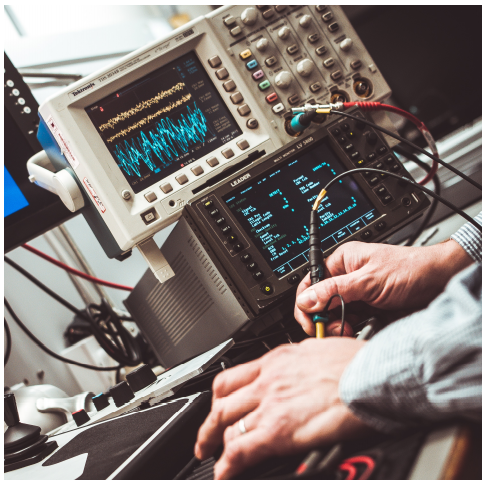
\includegraphics[scale=0.7]{portada.png}
\end{figure}

\hspace{1cm}
\begin{tabular}{|c| p{122mm}|}
	\hline
	\multirow{4}{50mm}{\\ \centering \large Apellidos y nombres}	 &  \\  
	& Alfaro Domínguez Rodrigo  \\  \cline{2-2}
	&  \\  
	& Barrera Peña Víctor Miguel \\  \cline{2-2}
	&  \\  
	& Villeda Hernández Erick Ricardo \\ 
	\hline
\end{tabular}
\begin{tabular}{|p{50mm} | c | p{80mm}| p{23mm} |}
	Grpo: & 4 & \multirow{2}{90mm}{Profesor: M.I Lauro Fernando Vazquez Alberto } & Calificación \\ \cline{1-2}
	Brigada: & 1 &  &\\ \hline
	Semestre: & 2021-1 & Fecha de ejecución: 22/09/2020-- 29/09/2020 & \\ \hline
\end{tabular}





	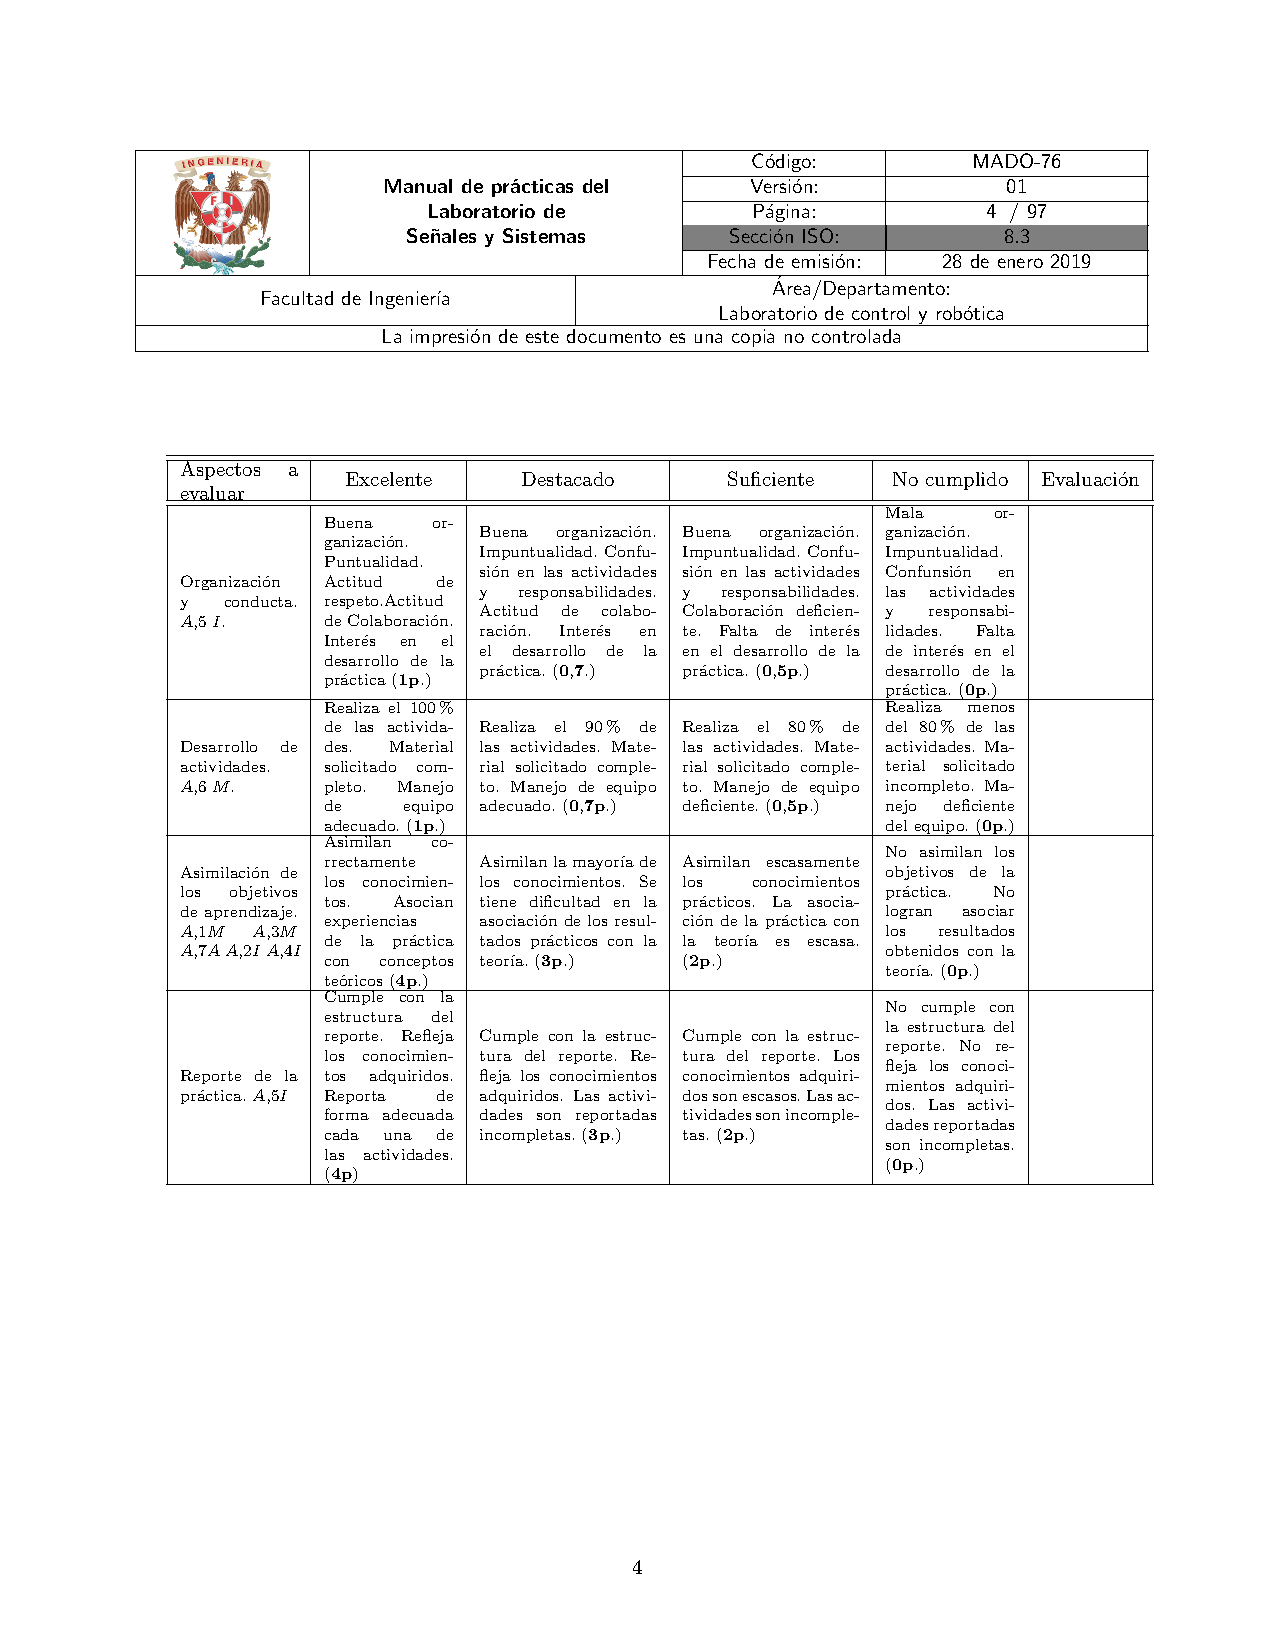
\includepdf[pages=-]{pdf/parte1.pdf}
	\noindent \justifying

\section{Previo}

\subsection{Identificar un sistema dinámico que se tenga en casa y definir la salida y la entrada del mismo (para discusión en clase)}
\subsection{¿Como analizaría un sistema de orden mayor?}
Para analizar un sistema de orden superior empezamos por escribir su función de transferencia:
\begin{equation}
H(s)=K\frac{(s-z_1)(s-z_2)...(s-z_n)}{(s-p_1)(s-p_2)(s-p_n)}
\end{equation} 
La mayor parte de la información de como funciona el ssitema nos la darán la localización de los polos y ceros. Esto determina si el sistema es estable o no.\\
En caso de tener polos reales la ecuación toma la siguiente forma:
\begin{equation}
H(s)=\frac{a_1}{s-p_1}+...+\frac{a_n}{s-p_n}
\end{equation}
A partir de aquí analizamos su respuesta a un impulso y un escalón, quedándonos sus ecuaciones de una de las siguientes formas respectivamente:
\begin{equation}
y_{imp}=\alpha_1 e^{p_1t}+..+\alpha_n e^{p_nt}
\end{equation}
\begin{equation}
y_{step}=\beta_0 + \beta_1 e^{p_1t}+...+ \beta_n e^{p_nt}
\end{equation}
Cada polo real p genera un término exponencial en la respuesta. El comportamiento de las osilaciones va a depender de si la parte real del poplo es negativa o positiva, mientras que la magnitud depende de los ceros.\\
En el caso de un sistema de segundo orden podemos escribir su ecuación característica en términos de zeta y omega, de la siguiente forma:
\begin{equation}
\frac{d^2y(t)}{dt^2}+2\zeta \omega_n \frac{dy(t)}{dt}+(\omega_n)^2y(t)=k(\omega_n)^2x(t)
\end{equation}
A partir de su respuesta en la ecuación homogénea podemos llegar a un polinimio de la siguiente forma:
\begin{equation}
s^2+2\zeta\omega_ns+\omega^2_n=0
\end{equation}
La respuesta del sistema va a depender de los valores que tenga el término $\zeta$, siendo sus valores posibles entre cero e infinito positivo. Lo que nos interesará para el diseño de un sistema es que su valor sea mayor o igual a uno.
\subsection{¿Cuál es la importancia de la constante de tiempo $\tau$ y el factor de amortiguamiento $\zeta$ ?}


\end{document}

